% This file was created with tikzplotlib v0.10.1.
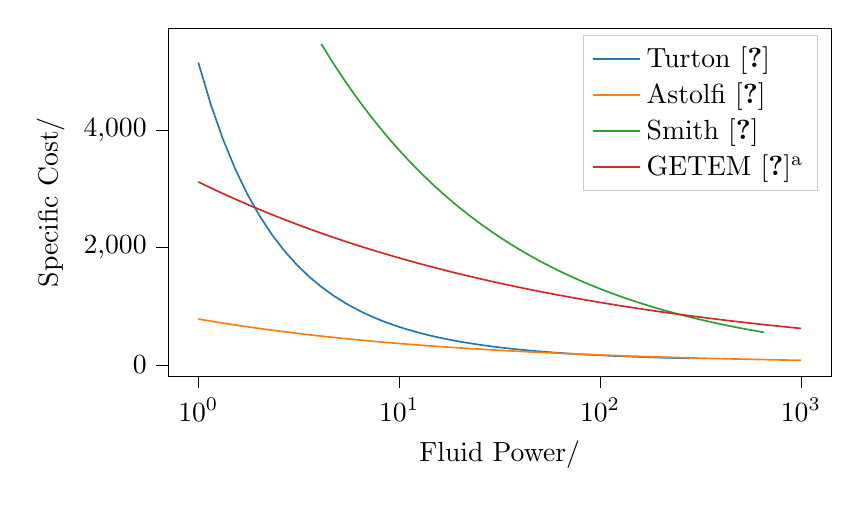
\begin{tikzpicture}

\definecolor{crimson2143940}{RGB}{214,39,40}
\definecolor{darkgray176}{RGB}{176,176,176}
\definecolor{darkorange25512714}{RGB}{255,127,14}
\definecolor{forestgreen4416044}{RGB}{44,160,44}
\definecolor{lightgray204}{RGB}{204,204,204}
\definecolor{steelblue31119180}{RGB}{31,119,180}

\begin{axis}[
legend cell align={left},
legend style={fill opacity=0.8, draw opacity=1, text opacity=1, draw=lightgray204},
log basis x={10},
tick align=outside,
tick pos=left,
unbounded coords=jump,
x grid style={darkgray176},
xlabel={Fluid Power/\unit{\kilo\watt}},
xmin=0.707945784384138, xmax=1412.53754462275,
xmode=log,
xtick style={color=black},
xtick={0.01,0.1,1,10,100,1000,10000,100000},
xticklabels={
  \(\displaystyle {10^{-2}}\),
  \(\displaystyle {10^{-1}}\),
  \(\displaystyle {10^{0}}\),
  \(\displaystyle {10^{1}}\),
  \(\displaystyle {10^{2}}\),
  \(\displaystyle {10^{3}}\),
  \(\displaystyle {10^{4}}\),
  \(\displaystyle {10^{5}}\)
},
y grid style={darkgray176},
ylabel={Specific Cost/\unit{\USD\per\kilo\watt}},
ymin=-189.32852892172, ymax=5742.72446479999,
ytick style={color=black}, 
width=10cm, height=6cm
]
\addplot [semithick, steelblue31119180]
table {%
1 5157.89778326774
1.15139539932645 4451.87660833814
1.32571136559011 3852.71182159373
1.52641796717523 3343.05061477957
1.75751062485479 2908.52230078589
2.02358964772516 2537.20094039359
2.32995181051537 2219.16885630982
2.68269579527973 1946.16139619631
3.08884359647748 1711.27725494923
3.55648030622313 1508.74179749058
4.09491506238043 1333.71331065815
4.71486636345739 1182.12409240525
5.42867543932386 1050.54986496538
6.25055192527397 936.10225949919
7.19685673001152 836.340128747398
8.28642772854684 749.196253130273
9.54095476349994 672.916655405196
10.9854114198756 606.010261699984
12.648552168553 547.207068041116
14.5634847750124 495.423311664648
16.7683293681101 449.732421540154
19.3069772888325 409.340745473163
22.2299648252619 373.567232099099
25.5954792269954 341.826393202871
29.4705170255181 313.613991621779
33.9322177189533 288.494997746567
39.0693993705462 266.09343752515
44.9843266896945 246.083820271431
51.7947467923121 228.183888206267
59.6362331659464 212.148473701606
68.66488450043 197.764286433949
79.060432109077 184.845482513024
91.0298177991522 173.229892298132
104.811313415469 162.775803991432
120.679264063933 153.359216971653
138.949549437314 144.87149282815
159.985871960606 137.2173436837
184.206996932672 130.313107071257
212.095088792019 124.085264695988
244.205309454865 118.46916914863
281.176869797423 113.407948268799
323.745754281764 nan
372.759372031494 nan
429.193426012878 nan
494.171336132383 nan
568.986602901829 nan
655.128556859551 nan
754.312006335462 nan
868.511373751352 nan
1000 nan
};
\addlegendentry{Turton \cite{Turton2012}}
\addplot [semithick, darkorange25512714]
table {%
1 784.82159191941
1.15139539932645 749.146683398902
1.32571136559011 715.093416167383
1.52641796717523 682.588076778086
1.75751062485479 651.56030250815
2.02358964772516 621.942929047865
2.32995181051537 593.671845113368
2.68269579527973 566.685853668073
3.08884359647748 540.926539452428
3.55648030622313 516.338142535258
4.09491506238043 492.867437612952
4.71486636345739 470.463618795255
5.42867543932386 449.078189628226
6.25055192527397 428.664858116333
7.19685673001152 409.179436516431
8.28642772854684 390.579745686702
9.54095476349994 372.825523783532
10.9854114198756 355.878339108657
12.648552168553 339.70150691794
14.5634847750124 324.260010011697
16.7683293681101 309.520422934671
19.3069772888325 295.45083962158
22.2299648252619 282.020804331611
25.5954792269954 269.201245722368
29.4705170255181 256.964413920551
33.9322177189533 245.28382045316
39.0693993705462 234.134180909188
44.9843266896945 223.491360207695
51.7947467923121 213.332320353765
59.6362331659464 203.635070569295
68.66488450043 194.378619690619
79.060432109077 185.542930729964
91.0298177991522 177.108877502364
104.811313415469 169.058203224132
120.679264063933 161.373480993297
138.949549437314 154.038076066437
159.985871960606 147.036109850261
184.206996932672 140.352425529993
212.095088792019 133.972555260155
244.205309454865 127.882688846725
281.176869797423 122.069643852886
323.745754281764 116.520837063649
372.759372031494 111.224257247576
429.193426012878 106.168439156659
494.171336132383 101.342438708052
568.986602901829 96.7358092939547
655.128556859551 92.3385791683423
754.312006335462 88.1412298616192
868.511373751352 84.1346755764496
1000 80.3102435201758
};
\addlegendentry{Astolfi \cite{Astolfi2014B}}
\addplot [semithick, forestgreen4416044]
table {%
1 nan
1.15139539932645 nan
1.32571136559011 nan
1.52641796717523 nan
1.75751062485479 nan
2.02358964772516 nan
2.32995181051537 nan
2.68269579527973 nan
3.08884359647748 nan
3.55648030622313 nan
4.09491506238043 5473.0856923581
4.71486636345739 5136.6648163292
5.42867543932386 4820.923135217
6.25055192527397 4524.58953556549
7.19685673001152 4246.47103700964
8.28642772854684 3985.44798957283
9.54095476349994 3740.46956617781
10.9854114198756 3510.54953222512
12.648552168553 3294.76227520793
14.5634847750124 3092.23907837948
16.7683293681101 2902.16462347157
19.3069772888325 2723.77370838475
22.2299648252619 2556.3481666362
25.5954792269954 2399.21397616383
29.4705170255181 2251.73854584692
33.9322177189533 2113.32816881965
39.0693993705462 1983.42563232483
44.9843266896945 1861.50797448575
51.7947467923121 1747.08437896527
59.6362331659464 1639.69419903651
68.66488450043 1538.90510311031
79.060432109077 1444.311334254
91.0298177991522 1355.5320766943
104.811313415469 1272.20992272848
120.679264063933 1194.00943387179
138.949549437314 1120.61579044852
159.985871960606 1051.7335241904
184.206996932672 987.085328739868
212.095088792019 926.410943269601
244.205309454865 869.46610472401
281.176869797423 816.021564464554
323.745754281764 765.862165360143
372.759372031494 718.785975607149
429.193426012878 674.603475791975
494.171336132383 633.13679592344
568.986602901829 594.21899936343
655.128556859551 557.69341077307
754.312006335462 nan
868.511373751352 nan
1000 nan
};
\addlegendentry{Smith \cite{Smith2005}}
\addplot [semithick, crimson2143940]
table {%
1 3122.3419350048
1.15139539932645 3021.44821917554
1.32571136559011 2923.81472983836
1.52641796717523 2829.33611774835
1.75751062485479 2737.91043786069
2.02358964772516 2649.43903932917
2.32995181051537 2563.82645905916
2.68269579527973 2480.98031870028
3.08884359647748 2400.81122496758
3.55648030622313 2323.23267318376
4.09491506238043 2248.16095393816
4.71486636345739 2175.51506276201
5.42867543932386 2105.21661272238
6.25055192527397 2037.18974984046
7.19685673001152 1971.36107124304
8.28642772854684 1907.65954595877
9.54095476349994 1846.01643827375
10.9854114198756 1786.36523356384
12.648552168553 1728.64156652345
14.5634847750124 1672.78315171367
16.7683293681101 1618.72971635451
19.3069772888325 1566.42293528891
22.2299648252619 1515.80636804826
25.5954792269954 1466.8253979516
29.4705170255181 1419.42717317266
33.9322177189533 1373.56054971132
39.0693993705462 1329.17603620779
44.9843266896945 1286.22574054006
51.7947467923121 1244.66331814697
59.6362331659464 1204.44392202115
68.66488450043 1165.52415431784
79.060432109077 1127.86201952744
91.0298177991522 1091.41687916115
104.811313415469 1056.14940790093
120.679264063933 1022.02155116642
138.949549437314 988.996484052946
159.985871960606 957.038571596437
184.206996932672 926.113330322328
212.095088792019 896.187391036923
244.205309454865 867.228462821105
281.176869797423 839.205298187542
323.745754281764 812.087659363782
372.759372031494 785.846285664854
429.193426012878 760.452861920178
494.171336132383 735.879987920713
568.986602901829 712.101148853365
655.128556859551 689.090686690774
754.312006335462 666.823772505586
868.511373751352 645.276379679352
1000 624.425257977141
};
\addlegendentry{GETEM \cite{GETEM2016}\textsuperscript{a}}
\end{axis}

\end{tikzpicture}
